\chapter{Simulation de l'environnement}
\chaptermark{Environnement}
\label{chapitre:environnement}
	
	\section{Introduction}

		Dans ce chapitre, nous allons nous intéresser à la simulation de l'environnement. Elle constitue une partie importante du simulateur car c'est elle qui va définir le comportement des \gls{ROV}s dans leur milieu.  A la fin de ce chapitre, nous devrions avoir à notre disposition un environnement de simulation complet proche de l'environnement rencontré lors de missions avec les robots.

		Pour ce faire, nous allons donc d'établir les différents élements de l'environnement qui vont interagir avec les \gls{ROV}s afin de les intégrer dans le simulateur. 
		
		Ce qui va principalement influencer le comportement des robots est le milieu marin qui va ajouter la flottabilité, les vagues, des courants marins et du vent. Ensuite, il y a l'ombilical qui relie les \gls{ROV}s au bateau afin de l'alimenter en énergie mais aussi d'avoir un retour d'informations. Enfin la présence de structures sous-marines jouent aussi un rôle importante dans les missions des \gls{ROV}s, que ce soit par exemple des piles d'éolienne à inspecter pour le robot \argos{}, son garage, ou bien des structures sous-marines à deplacer pour \atoll{}.

		Nous allons donc nous intéresser par la suite a la manière de simuler ces différents éléments d'environnement pour le simulateur.

		% La \textsc{Table}~\ref{table:elements} présente les différents élements cités précédemment qui peuvent être simulés dans un environnement marin. Nous allons choisir les principaux car tous n'auront pas un impact significatif sur le comportement des \gls{ROV}s, comme le vent ou les vagues. 

		% \begin{table}[ht]
		% 	\centering
		% 	\begin{tabular}{|c|c|}
		% 		\hline
		% 		\textbf{Elément} & \textbf{Simulation} \\
		% 		\hline
		% 		Vent & \xmark\\
		% 		\hline
		% 		Vagues & \xmark\\
		% 		\hline
		% 		Courant marins & \cmark \\
		% 		\hline
		% 		Ombilical & \cmark \\
		% 		\hline
		% 		Garage d'\argos{} & \cmark \\
		% 		\hline
		% 		\gls{frameLBL} & \cmark \\
		% 		\hline
		% 		Pile d'éolienne & \cmark \\
		% 		\hline
		% 	\end{tabular}
		% 	\caption{Elements pris en compte dans l'environnement de simulation}
		% 	\label{table:elements}
		% \end{table}

	\section{Environnement marins}

		\section{Courants marins}

			Les courants marins constituent un élément majeur qui va perturber le comportement des robots dans l'environnement simulé. Avec une simulation suffisament précise, la simulation et le comportement réel des \gls{ROV}s deviendront très proches, notamment par l'ajout de la traînée hydrodynamique qui va s'appliquer sur les composants des robots.

			\subsection{Modèle constant}

				Pour simuler ces courants, il est possible d'utiliser en première approximation une idée assez triviale : localement le courant est constant. Par constant on entend uniforme, donc qui ne dépend pas de l'espace, et stationnaire, donc qui ne dépend pas du temps. C'est à dire qu'il est possible de considérer le courant marin  comme un champ de vecteurs ayant un certain cap et une certaine magnitude représentant la vitesse de l'écoulement. Ce modèle simple permet de rapidement ajouter du courant dans notre simulateur, mais ce courant est peu réaliste dans la mesure ou il ne prends pas du tout en compte la présence de structures sous-marine qui pourraient modifier la vitesse et l'orientation de ce courant, comme les piles d'éoliennes ou bien les structures sous marines à déplacer.

				\begin{figure}[!htb]
					\centering
					\inputpgf{imgs/pgf}{constant.pgf}
					\caption{Modèle de courant constant}
					\label{fig:constant}
				\end{figure}

			\subsection{Modèle procédural}

				Une autre idée serait de générer un courant pseudo-aléatoire par génération procédurale. Cette méthode de génération est largement utilisée dans le domaine des jeux-vidéos et du cinéma, et par extension, il est aussi utilisé dans le domaine de la simulation~\cite{generation_procedurale_monde, volumetric_terrain_generation}. Elle permet de générer à l'aide d'algorithme des mondes et des textures pseudo-aléatoires. Dans notre cas, il est possible d'utiliser le \textit{Bruit de Perlin}~\cite{PerlinNoise} qui est une texture procédurale afin de générer des courants. L'avantage du \textit{Bruit de Perlin} est qu'il est très peu coûteux en espace mémoire et qu'il peut générer des textures dans n'importe quelle dimensions. 
				
				Pour notre application nous pouvons générer une texture en deux dimensions. Cette texture forme un potentiel artificiel, et un champ de vecteur représentant le courant peut être simplement généré en prenant le gradiant de ce potentiel. On obtient le résultat présenté en \textsc{Figure}~\ref{fig:perlin_noise}. Comme avec cette méthode, chaque pixel tient compte de ses pixels voisins, on ne se retrouve pas avec des valeurs très éloignées entre deux pixels adjacents comme avec de la génération de textures purement aléatoire, et on obtient des courants réalistes.

				\begin{figure}[!htb]
					\centering
					\begin{subfigure}[b]{0.32\textwidth}
						\centering
						\inputpgf{imgs/pgf/}{random.pgf}
						\caption{Bruit aléatoire}
					\end{subfigure}
					\hfill
					\begin{subfigure}[b]{0.32\textwidth}
						\centering
						\inputpgf{imgs/pgf/}{perlin.pgf}
						\caption{Bruit de Perlin}
					\end{subfigure}
					\hfill
					\begin{subfigure}[b]{0.32\textwidth}
						\centering
						\inputpgf{imgs/pgf/}{courant.pgf}
						\caption{Courant généré}
					\end{subfigure}
					\caption{Comparaison bruit aléatoire et bruit de Perlin}
					\label{fig:perlin_noise}
				\end{figure}

				C'est une bonne approche pour générer des courants marins de manière pseudo-aléatoire, mais il est difficile de reproduire de manière contrôlée les courants marins qu'il y aurait eu lors d'un essai en milieu naturel afin de comparer les résultats de la simulation avec le comportement des \gls{ROV}s réels.
				
				Il serait cependant intéressant d'utiliser ce genre d'algorithme pour de la génération procédurale de terrain. En effet, en interpretant la carte 2D comme un modèle d'élévation numérique de terrain, on serait en mesure de créer de manière pseudo-aléatoire des fonds marins pour testers les robots dans différents environnements.

			\subsection{Modèle de Navier-Stokes}

				Une simulation des courants marins basée sur les équations de Navier-Stokes permet de proposer une approche intéressante à la simulation de courants marins~\cite{Garau2006current}. Ils permettent notament de générer des courants prenant en compte la présence de solides dans le milieu à explorer, comme des rochers ou des piles d'éoliennes offshores qui peuvent être intéressante pour notre application. C'est la méthode qui fournirait les résultats les plus vraisemblables et les plus proche de ce qu'on pourrait trouver en milieu naturels.

				En revanche les équations de Navier-Stokes sont des équations aux dérivées partielles non-linéaires~\cite{hinch2012hydrodynamique} qui sont lourdes à résoudre numériquement. Elles alourdiraient grandement la simulation afin de calculer le courant en chaque point de l'espace afin d'impacter tous les solides constituants les robots mais aussi les éléments de l'environnement comme les structures sous-marines et les ombilicaux par exemple.

			\subsection{Choix du modèle}

				Il faut maintenant choisir un modèle qui va être implémenté dans le simulateur. Pour nous aider dans ce choix, la \textsc{Table}~\ref{table:courants} reprends les principales caractéristiques des différents modèles, à savoir le caractèr non-aléatoire des courants générés et la prise en compte des structures sous-marines. Le réalisme des courants générés ainsi que la complexité d'implémentation est aussi présentée. Cette dernière représente à la fois le temps d'implémentation de la solution ainsi que la complexité d'execution de celle-ci en terme de ressources nécéssaires. Elle est représentée par le symbole \pmark (\pmark : \textit{simple}, \pmark \pmark : \textit{intermédiaire}, \pmark \pmark \pmark : \textit{complexe}).

				\begin{table}[ht]
					\centering
					\begin{adjustbox}{max width=\textwidth}
						\begin{tabular}{|c|c|c|c|c|}
							\hline
							\textbf{Modèle de courants} & \textbf{Non aléatoire} & \textbf{Structures sous-marines} & \textbf{Réalisme} & \textbf{Complexité} \\
							\hline
							Modèle constant & \cmark & \xmark & \pmark \pmark & \pmark\\
							\hline
							Modèle procédural & \xmark & \xmark & \pmark & \pmark \pmark \\
							\hline
							Modèle Navier-Stokes & \cmark & \cmark & \pmark \pmark \pmark & \pmark \pmark \pmark \\
							\hline
						\end{tabular}
					\end{adjustbox}
					\caption{Différents modèles de simulation de courants}
					\label{table:courants}
				\end{table}

				Nous pouvons aisement écarter le modèle procédural car on remarque au vu des éléments présentés sur la \textsc{Table}~\ref{table:courants} qu'il n'est pas adapté à notre simulateur. Quant au modèle de Navier-Stokes, il est bien trop lourd à mettre en place, et les calculs sont très coûteux en terme de ressources pour une simulation temps réel. Notre choix se porte donc l'utilisation du modèle constant dans la mesure où il fournit un niveau de réalisme suffisant à l'échelle macroscopique qui est intéressante dans notre application, pour un niveau de complexité très faible. Il faudra tout de même garder à l'esprit que le modèle ne prends pas en compte les courants, ce qui constitue une limite pour notre simulateur.

		\section{Simulation d'ombilicaux}

			\subsection{Etat de l'art}

			\subsection{Formalisme}

				Supposons que nous voulons simuler un ombilical de longueur $L$. On va alors le diviser en un nombre fini de n\oe uds $n$ connectés par des liens. Ces liens doivent donc avoir une longueur $l=\frac{L}{n-1}$.
			
				Pour cette simulation, nous allons prendre en compte le poids noté $\overrightarrow{P}$, la flottabilité notée $\overrightarrow{\Pi}$, la force exercée par l'élément précédant sur l'élément considéré notée $\overrightarrow{F_p}$, tout comme celle exercée par l'élément suivant notée $\overrightarrow{F_s}$, et enfin la force de frottements fluides notée $\overrightarrow{F_f}$.
				
				\begin{description}
					\item [Bilan des Forces] \
					\begin{itemize}
						\item[\textbullet] \textbf{Poids $\overrightarrow{P}$} : En considérant que chaque élément a une masse $m$, et en notant $g$ l'accélération de pesanteur, on a : 
						
						\begin{equation}
							\overrightarrow{P} = \begin{bmatrix}0\\ 0\\ -m.g\end{bmatrix}
							\label{eq:poids}
						\end{equation}
				
						\item[\textbullet] \textbf{Poussée d'Archimède $\overrightarrow{\Pi}$} : Si on note le volume d'un élément $V$ et $\rho$ la masse volumique du fluide dans lequel est immergé l'ombilical, on a : 
						
						\begin{equation}
							\overrightarrow{\Pi} = \begin{bmatrix}0\\ 0\\ \rho.V.g\end{bmatrix}
							\label{eq:archimede}
						\end{equation}
				
						\item[\textbullet] \textbf{Trainée hydrodynamique $\overrightarrow{F_f}$} : En notant $A$ la surface de référence, $C_D$ le coefficient de trainée, $\rho$ la masse volumique du fluide, et $\overrightarrow{v}$ la vitesse du n\oe ud, on a : 
					
						\begin{equation}
							\overrightarrow{F_f} = - \frac{1}{2} \cdot \rho \cdot A \cdot C_D \cdot ||\overrightarrow{v}|| \cdot \overrightarrow{v}
							\label{eq:drag}
						\end{equation}
						
						\item[\textbullet] \textbf{Force inter-éléments $\overrightarrow{F_p}$ et $\overrightarrow{F_s}$} : Il est difficile de trouver une forme analytique pour décrire cette force. Nous avons toutefois trouver un moyen de l'exprimer. C'est pourquoi nous allons utiliser ici un modèle comportemental de ces forces. Nous savons que chaque n\oe ud doit se trouver à une distance $l$ de ses voisins. En notant $p_{p}$ la position du n\oe ud précédent et $p_{c}$ la position du n\oe ud considéré, en introduisant les trois coefficients $K_p$, $K_d$ et $K_i$ qui vont nous permettre de régler la dynamique du système, on est en mesure de proposer le modèle de force comportemental suivant :
						
						\begin{equation}
							\overrightarrow{F} = - \left(K_p \cdot e(t) + K_d \cdot \dot e(t) + K_i \cdot \int_{0}^te(\tau) \cdot d\tau \right) \cdot \overrightarrow{u}
							\label{eq:pid}
						\end{equation}
						
						Dans cette expression, $\overrightarrow{u}$ est le vecteur unitaire orienté du n\oe ud courant vers le n\oe ud voisin, $e$ est l'erreur de positionnement du n\oe ud, $\dot e$ est la dérivée de cette erreur et $\int_{0}^te(\tau) \cdot d\tau$ est l'intégrale de cette erreur. La dérivée et l'intégrale de cette erreur sont estimées numériquement en utilisant respectivement la méthode d'Euler et la méthode des rectangle. On trouve les expressions de $\overrightarrow{u}$ et $e(t)$ pour deux éléments en position $\mathbf{p_c}$ et $\mathbf{p_p}$ tel que $||\mathbf{p_c} - \mathbf{p_p}|| \neq 0$ :

						\begin{equation}
							\overrightarrow{u} = \frac{\mathbf{p_c} - \mathbf{p_p}}{||\mathbf{p_c} - \mathbf{p_p}||} \qquad e(t) = \frac{||\mathbf{p_c} - \mathbf{p_p}|| - l}{||\mathbf{p_c} - \mathbf{p_p}||}
							\label{eq:behavioral}
						\end{equation}
						
						Les deux forces $\overrightarrow{F_p}$ et $\overrightarrow{F_s}$ peuvent enfin être exprimées en utilisant l'expression de $\overrightarrow{F}$ et en prenant soin d'adapter les expressions de $\overrightarrow{u}$ et $e(t)$ en actualisant l'élément courant et l'élément précédent.
					\end{itemize}
				\end{description}
			
				Ainsi on a exprimé les forces nécéssaires à la simulation de l'ombilical par éléments finis. La \textsc{Figure}~\ref{fig:modelization} montre la modélisation du problème. Les différents n\oe uds sont représentés en bleu. Pour des raisons de clarté, les différentes forces ne sont représentées que sur un seul n\oe ud mais sont bien évidemment appliquées sur tous les n\oe uds, et la représentation de l'ombilical est volontairement tronquée.
			
				\begin{figure}[!htb]
					\centering
					\begin{tikzpicture}
						\tikzstyle{TetherElement}=[circle,draw,fill=RoyalBlue]
						\tikzstyle{Link}=[thick,black]
						\tikzstyle{vector}=[-stealth,Red,very thick]
						\tikzset{ext/.pic={
							\path [fill=white] (-0.2,0)to[bend left](0,0.1)to[bend right](0.2,0.2)to(0.2,0)to[bend left](0,-0.1)to[bend right](-0.2,-0.2)--cycle;
							\draw (-0.2,0)to[bend left](0,0.1)to[bend right](0.2,0.2) (0.2,0)to[bend left](0,-0.1)to[bend right](-0.2,-0.2);
						}}
			
						\foreach \x in {1, 2, 3, 4, 5}
							\node[TetherElement] (T\x) at ({1.5*(\x-3)+3.5}, {8*cosh(0.25*(\x-3))-7}) {};
			
						\draw[Link] (T1) -- pic[rotate=45,scale=0.6] {ext} (T2);
						\draw[Link] (T2) -- (T3) -- (T4);
						\draw[Link] (T4) -- pic[rotate=-70,scale=0.6] {ext} (T5);
						
						\node (fp) at ($(T2)!.3!(T3)$) {};
						\draw[vector] (T3) -- (fp) node[yshift=1em]{$\overrightarrow{F_p}$};
			
						\node (fn) at ($(T3)!.7!(T4)$) {};
						\draw[vector] (T3) -- (fn) node[yshift=1em]{$\overrightarrow{F_n}$};
						\draw[vector] (T3) -- +(270:1cm) node[yshift=-.6em]{$\overrightarrow{P}$};
						\draw[vector] (T3) -- +(90:1cm) node[yshift=.6em]{$\overrightarrow{\Pi}$};
						\draw[vector] (T3) -- +(225:0.8cm) node[xshift=-.5em]{$\overrightarrow{F_f}$};
						\draw[vector,Green] (T3) -- +(45:1cm) node[xshift=.2em,yshift=.4em]{$\overrightarrow{v}$};
			
						\draw[->,red,very thick] (0,0) -- (-0.4,-0.6) node[left] {$\mathbf{x}$}; 
						\draw[->,Green,very thick] (0,0) -- (1,0) node[above left] {$\mathbf{y}$}; 
						\draw[->,blue,very thick] (0,0) -- (0,1) node[above] {$\mathbf{z}$}; 
					\end{tikzpicture}
					\caption{Modelization of the problem}
					\label{fig:modelization}
				\end{figure}
			
			
			\subsection{Initialisation}
				L'initialisation des différents n\oe uds de l'ombilical est une étape importante car les coefficients du modèle comportemental sont reglés pour avoir un comportement cohérent lorsque la position du câble a convergée. Si l'initialisation est aléatoire, le temps du régime transitoire peut être long et la simulation peut ne pas être consistante. De plus il faut impérativement que deux n\oe uds adjacents n'aient pas la même position, sinon l'expression de $\overrightarrow{u}$ dans l'\textsc{Equation}~\ref{eq:behavioral} n'est plus valable, car le dénominateur n'annule.
			
				Pour initialiser l'ombilical, nous allons nous appuyer sur l'équation de la chaînette. Cette équation représente la forme que prend une corde attachée à ses deux extrémités, sachant qu'elle va chercher à minimiser son énergie potentielle [? ref ?]. L'équation de la chaînette est valable pour une corde attachée à ses extrémités en $(-x_0, y_0, z_0)$ et $(x_0, y_0, z_0)$.
				
				Dans notre cas, notre ombilical va pouvoir être attaché à deux extrémités aux positions $p_1 = (x_1, y_1, z_1)$ et $p_n = (x_n, y_n, z_n)$ qui peuvent être quelconque, nous allons devoir ajouter deux coefficients $c_2$ et $c_3$ à la solution de l'équation de la chaînette permettants de translater sa représentation graphique dans le plan. Ainsi la forme que va prendre notre obilical lors de l'initialisation va être régie par l'\textsc{Equation}~\ref{eq:tether}.
			
				\begin{equation}
					z = c_1\cdot cosh\left(\frac{x + c_2}{c_1}\right) + c_3
					\label{eq:tether}
				\end{equation}
			
				Il nous reste à estimer les trois paramètres $c_1$, $c_2$ et $c_3$ introduits à partir des conditions aux limites. Les contraintes sont telles que les deux extremités de l'ombilical doivent se trouver en $p_1$ et en $p_n$, et le câble doit avoir une longueur $L$. Ces trois contraintes se traduisent par le système non-linéaire de trois équations à trois inconnues présenté en \textsc{Equation}~\ref{eq:systeme} à résoudre.
				
				\begin{align}
					S_1 = 
					\begin{cases}
						L   = & c_1 \cdot sinh\left(\dfrac{x_n+c_2}{c_1}\right) - c_1 \cdot sinh\left(\dfrac{x_1+c_2}{c_1}\right) \\
						z_1 = & c_1 \cdot cosh\left(\dfrac{x_1+c_2}{c_1}\right)+c_3 \\
						z_n = & c_1 \cdot cosh\left(\dfrac{x_n+c_2}{c_1}\right)+c_3
					\end{cases}
					\label{eq:systeme}
				\end{align}
			
				\begin{figure}[!htb]
					\centering
					\begin{subfigure}[b]{0.45\textwidth}
						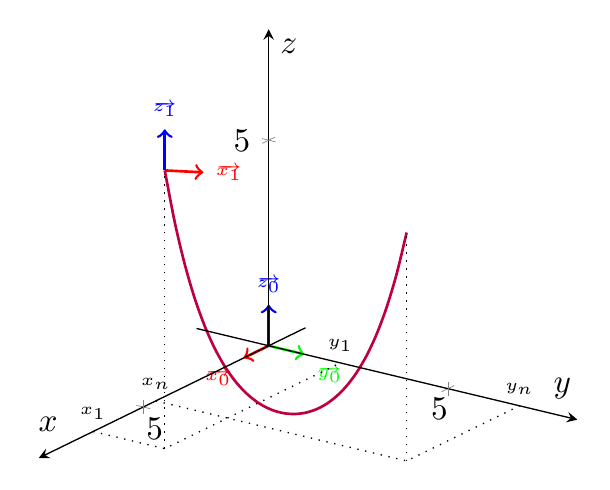
\begin{tikzpicture}[scale=1.2]
							\begin{axis}[view={125}{20},
								axis lines=center,axis on top,
								xlabel=$x$,ylabel=$y$,zlabel=$z$,
								no marks,axis equal,
								xmin=0,xmax=7,ymin=0,ymax=6,zmin=0,zmax=7,
								enlargelimits={upper=0.1}]
				
								% R0
								\draw[thick,->, red] (0,0,0) -- (1,0,0) node[anchor=north east] (x0) {\tiny $\overrightarrow{x_0}$};
								\draw[thick,->, green] (0,0,0) -- (0,1,0) node[anchor=north west] (y0) {\tiny $\overrightarrow{y_0}$};
								\draw[thick,->, blue] (0,0,0) -- (0,0,1) node[anchor=south] (z0) {\tiny $\overrightarrow{z_0}$};
				
								% R1
								\draw[thick,->, red] (7,2,6.769) -- ++(-0.4,0.8,0) node[anchor=west] (x1) {\tiny $\overrightarrow{x_1}$};
								\draw[thick,->, blue] (7,2,6.769) -- ++(0,0,1) node[anchor=south] (z1) {\tiny $\overrightarrow{z_1}$};
				
								% Tether
								\addplot3[
									samples y=0,
									smooth, thick, color=purple,
									domain=2:7
									] ({8-0.5*x},{x},{cosh(x-4.6)});
								
								% label points
								\node [above] at (7,0,0) {\tiny $x_1$};
								\node [above] at (0,2,0) {\tiny $y_1$};
								\node [above] at (4.5,0,0) {\tiny $x_n$};
								\node [above] at (0,7,0) {\tiny $y_n$};
				
								% Dots
								\draw[dotted] (7,0,0) -- (7,2,0) -- (0,2,0);
								\draw[dotted] (7,2,0) -- (7,2,6.769);
								
								\draw[dotted] (4.5,0,0) -- (4.5,7,0) -- (0,7,0);
								\draw[dotted] (4.5,7,0) -- (4.5,7,5.556);
							\end{axis}
						\end{tikzpicture}
						\caption{Dans le repère du monde}
						\label{fig:3d_plot}
					\end{subfigure}
					\hfill
					\begin{subfigure}[b]{0.45\textwidth}
						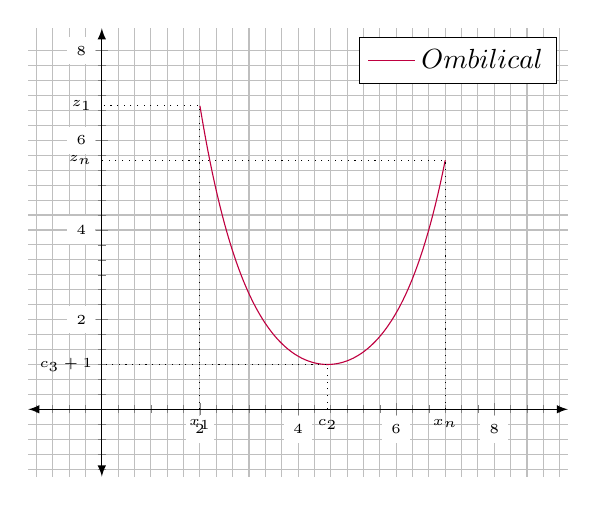
\begin{tikzpicture}
							\begin{axis}[
									xmin=-1,   xmax=9,
									ymin=-1,   ymax=8,
									grid=both,
									axis lines=middle,
									minor tick num=5,
									enlargelimits={abs=0.5},
									axis line style={latex-latex},
									ticklabel style={font=\tiny,fill=white},
									xlabel style={at={(ticklabel* cs:1)},anchor=north west},
									ylabel style={at={(ticklabel* cs:1)},anchor=south west}
								]
								\addplot [
									domain=2:7, 
									samples=100, 
									color=purple,
									]
									{cosh(\x - 4.6)};
								\addlegendentry{$Ombilical$}
			
								% Labels
								\node[below] at (2,0) {\tiny $x_1$};
								\node[below] at (7,0) {\tiny $x_n$};
								\node[left] at (0,6.769) {\tiny $z_1$};
								\node[left] at (0,5.556) {\tiny $z_n$};
								\node[left] at (0,1) {\tiny $c_3 + 1$};
								\node[below] at (4.6, 0) {\tiny $c_2$};
			
								% Dots
								\draw[dotted] (2,0) -- (2,6.769) -- (0,6.769);
								\draw[dotted] (4.6,0) -- (4.6,1) -- (0,1);
								\draw[dotted] (7,0) -- (7,5.556) -- (0,5.556);
							\end{axis}
						\end{tikzpicture}
						\caption{Dans le repère de l'ombilical}
						\label{fig:2d_plot}
					\end{subfigure}
					\caption{Modélisation de l'ombilical en 3 dimensions}
					\label{fig:tether_plot}
				\end{figure}
				
				Pour résoudre ce système et trouver une approximation numérique pour $c_1$, $c_2$ et $c_3$, on utilise un solveur numérique. Lors de l'implémentation pour le simulateur de cette étape d'initialisation, la librairie \gls{GSL}\footnote{\url{https://www.gnu.org/software/gsl/}} est utilisée. Une fois les paramètres déterminés, on est en mesure de déterminer la position initiale de chaque n\oe ud dans le repère de l'ombilical. Il faut enfin projeter ces positions dans le repère du monde afin de pouvoir correctement initialiser chaque n\oe uds, comme présenté sur la \textsc{Figure}~\ref{fig:tether_plot}
			
			\subsection{Implémentation}
				L'implémentation d'un \plugin{} \gazebo{} permet de simuler le comportement de l'ombilical dans l'environnement de simulation. Ce \plugin{} est basé sur l'instanciation d'objets de type \textit{Tether} et \textit{TetherElement}. L'objet \textit{Tether} possède les paramètres de simulation de l'ombilical, tandis que l'objet \textit{TetherElement} représente un tronçon de cet ombilical. Un diagramme de classe est présenté en \textsc{Figure}~\ref{fig:uml_class} et montre les différents attributs et méthodes associées à chaque classe.

				\begin{figure}[!htb]
					\centering
					\resizebox{0.50\textwidth}{!}{
						\begin{tikzpicture}
							\begin{class}[text width=6cm]{Tether}{0,0}
								\attribute{+ element\_mass : double}
								\attribute{+ element\_volume : double}
								\attribute{+ element\_length : double}
								\attribute{+ position\_first : numpy.ndarray}
								\attribute{+ position\_last : numpy.ndarray}
								\attribute{+ elements : list of \textit{TetherElement}}
							\end{class}
						
							\begin{class}[text width=6cm]{TetherElement}{8.5,0}
								\attribute{+ mass : double}
								\attribute{+ volume : double}
								\attribute{+ length : double}
								\attribute{+ position : numpy.ndarray}
								\attribute{+ velocity : numpy.ndarray}
								\attribute{+ acceleration : numpy.ndarray}
								\attribute{+ previous : TetherElement}
								\attribute{+ next : TetherElement}
								\attribute{+ K\_p : double}
								\attribute{+ K\_d : double}
								\attribute{+ K\_i : double}
								\operation{+ F\_p(self) : numpy.ndarray}
								\operation{+ F\_b(self) : numpy.ndarray}
								\operation{+ F\_f(self) : numpy.ndarray}
								\operation{+ Ft\_prev(self) : numpy.ndarray}
								\operation{+ Ft\_next(self) : numpy.ndarray}
							\end{class}
						
							\aggregation{Tether}{}{~~~n}{TetherElement}
						\end{tikzpicture}
					}
					\caption{Diagramme de classe UML des classes \textit{Tether} et \textit{TetherElement}}
					\label{fig:uml_class}
				\end{figure}
				
				La \textit{Tether} utilise une structure de \textit{liste doublement chaînée}\footnote{structure de données liée qui consiste en un ensemble n\oe uds liés les uns aux autres par des références au n\oe uds voisins.} de \textit{TetherElement}. Chaque \textit{TetherElement} possède alors une référence vers l'élément le précédant et l'élément le suivant, comme le montre la \textsc{Figure}~\ref{fig:doubly_linked_list}. La \textit{Tether} ne possède ainsi qu'une référence vers le premier et le dernier n\oe ud de la chaîne, nommés respectivements \textit{head} et \textit{tail}. Il est ensuite possible de parcourir la chaîne de \textit{TetherElement} dans les deux sens en utilisant les références gardées par les \textit{TetherElement} eux-mêmes. 
			
				\begin{figure}[!htb]
					\centering
					\resizebox{0.90\textwidth}{!}{
						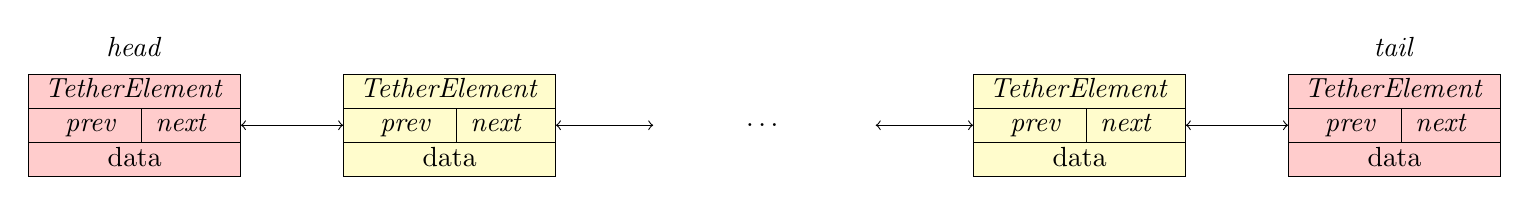
\begin{tikzpicture}
							\tikzset{TE/.style={draw, inner sep=0, outer sep=0, fill=yellow!20}}
			
							\node[TE, fill=red!20] (TE0) at (0,0) {\begin{tabular}{c} \textit{TetherElement} \\ \hline \hfill \textit{prev} \hfill \vline \hfill \textit{next} \hfill \\ \hline data \end{tabular}};
			
							\node[TE, fill=red!20] (TE4) at (16,0) {\begin{tabular}{c} \textit{TetherElement} \\ \hline \hfill \textit{prev} \hfill \vline \hfill \textit{next} \hfill \\ \hline data \end{tabular}};
			
							\foreach \i in {1,3} {
								\node[TE] (TE\i) at (4*\i,0) {\begin{tabular}{c} \textit{TetherElement} \\ \hline \hfill \textit{prev} \hfill \vline \hfill \textit{next} \hfill \\ \hline data \end{tabular}};
							}
							\node[minimum width=80] (TE2) at (8,0) {\dots};
							\foreach \i in {0,1,2,3} {
								\pgfmathtruncatemacro{\next}{\i +1}
								\draw[<->] (TE\i) -- (TE\next);
							}
			
							\node (head) at (0,1) {\textit{head}};
							\node (tail) at (16,1) {\textit{tail}};
						\end{tikzpicture}
					}
					\caption{Liste doublement chainée}
					\label{fig:doubly_linked_list}
				\end{figure}

				A chaque pas de temps, on va actualiser la position des \textit{TetherElement}. Les extrémités peuvent être libres, dans ce cas on les traites comme les autres \textit{TetherElement}, ou bien attachée à des solides, dans ce cas la position actualisée est celle de l'élément auquel l'extrémité est attachée. Puis, on parcours la \textit{liste doublement chaînée} et on réalise le bilan des forces qui s'appliquent sur chaque éléments. D'après le Principe Fondamental de la Dynamique, en notant $a$ l'accélération d'un \textit{TetherElement}, on a :

				\begin{equation}
					m.a_{t_{i+1}} = \overrightarrow{P} + \overrightarrow{\Pi} + \overrightarrow{F_f} + \overrightarrow{F_p} + \overrightarrow{F_s}
					\label{eq:newton}
				\end{equation}

				A ce stade, on peut appliquer l'accélération des \textit{TetherElement} aux extrémités dans les solides auxquel l'ombilical est attaché. Par exemple si l'ombilical simulé est attaché à un robot, il va induire une force à celui-ci qui va le gêner dans ses mouvements. Cette force est égale à l'opposé de la somme des forces calculées dans l'élément en extrémité d'ombilical.
				
				Ensuite, à l'aide de la méthode d'Euler on est en mesure d'obtenir une approximation de la vitesse puis de la position de chaque éléments. En notant $v$ la vitesse et $p$ la position d'un \textit{TetherElement}, et $h$ le pas de temps entre deux instants de calculs, on a :

				\begin{eqnarray}
					v_{t_{i+1}} & = & v_{t_i} + h.a_{t_{i+1}} \\
					p_{t_{i+1}} & = & p_{t_i} + h.v_{t_{i+1}}
					\label{eq:euler}
				\end{eqnarray}

				On a donc actualisé la position de chaque \textit{TetherElement}. Après avoir actualisé la représentation graphique de cet élément dans \gazebo{}, on est prêt pour la prochaine itération de calcul.
			
			\subsection{Suivi d'angles normalisés}
				Un problème avec la représentation numérique de l'orientation des solides est qu'elle est souvent normalisée, et les valeurs sont ainsi ramenées dans l'intervalle $[-\pi; \pi]$. On ne peut donc pas avoir l'orientation absolue, c'est à dire l'orientation d'un solide en prenant en compte les eventuels tours qu'il aurait pu faire sur lui-même. C'est le cas dans \gazebo{}, et cela pose problème pour le calcul du couple transmissible le long de l'ombilical qui utilise l'orientation absolue des \textit{TetherElements}.
			
				Pour résoudre ce problème, l'\textsc{Algorithme}~\ref{algo:suivi_angle} de suivi d'angles normalisés a été implémenté. Il prends en paramètres l'angle normalisé ainsi que l'angle précédemment calculé, et il retourne la valeur de l'angle absolu. L'idée de fournir l'angle précédent est de pouvoir retourner le nouvel angle qui se trouve dans le même quadrant et aussi de pouvoir suivre les sauts d'angles. Ainsi on peut suivre l'orientation absolue de solides en rotation dans l'espace, en ne fournissant que des orientations relatives ramenées dans l'intervalle $[-\pi; \pi]$, et en gardant en mémoire la précédente orientation calculée.
				
				\begin{algorithm}[!htb]
					\SetKwInOut{Input}{Entrées}
					\SetKwInOut{Output}{Sorties}
					\Entree{$angle\_normalise$, $angle\_absolu$}
					\Sortie{$angle\_absolu$}
					\Deb{
						$offset \leftarrow (angle\_absolu - angle\_normalise + \pi ) \pmod{2\pi}$ \\
						$angle\_absolu \leftarrow angle\_normalise + 2\pi \cdot offset$ \\
					}
					\Retour{$angle\_absolu$}
			
					\caption{Suivi d'angle} 
					\label{algo:suivi_angle}
				\end{algorithm}
			
				La \textsc{Figure}~\ref{fig:suivi_angle} présente les résultats de l'\textsc{Algorithme}~\ref{algo:suivi_angle} avec une angle variant dans l'intervalle $[-3\pi; 3\pi]$. On voit sur la première sous-figure l'angle réel et l'angle ramené dans l'intervalle $[-\pi; \pi]$ avec la présence de saut d'angles. Avec cette méthode, on est capable de suivre l'évolution de l'angle et de supprimer ces sauts afin de retrouver l'angle absolu visible dans la deuxième sous-figure et calculé uniquement à partir de la connaissance de l'angle normalisé. Cet algorithme ne marche en revanche que pour une variation d'angle continue, car en cas de saut brusque d'angle les tours ajoutés ne seront pas pris en compte.
			
				\begin{figure}[!htb]
					\centering
					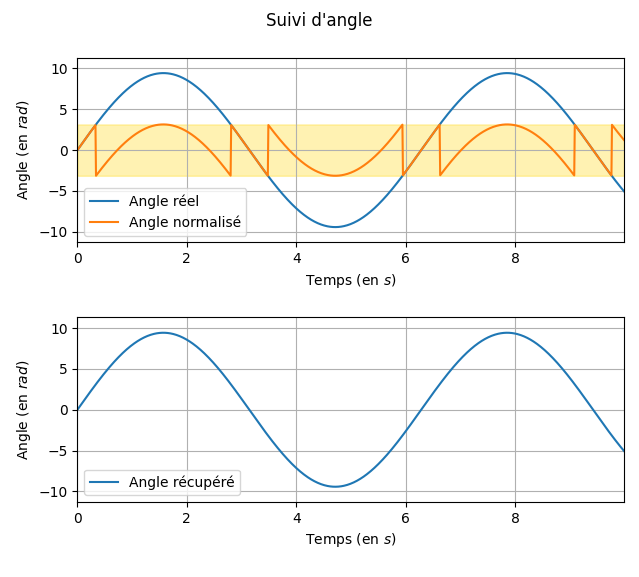
\includegraphics[width=0.5\textwidth]{suivi_angle.png}
					\caption{Suivi d'angle}
					\label{fig:suivi_angle}
				\end{figure}		
		
		\subsection{Resultats}

		\section{Garage d'\argos{}}

		\section{Structures sous-marines}
		